undefined
\begin{document}

\title{Targeted Adversarial Examples for Air Traffic Speech Recognition}

\author{
  Andrew Dassonville\\
  \texttt{dassonva@oregonstate.edu}
  \and
  Austin Friedrich\\
  \texttt{friedrau@oregonstate.edu}
  \and
  Matthew Brayton\\
  \texttt{braytonm@oregonstate.edu}
}

\maketitle

\thispagestyle{firstpage}

\begin{abstract}
  We present a novel technique designed specifically for generating targeted
  adversarial examples aimed at compromising air traffic speech recognition
  systems. This method is leveraged to create adversarial pilot weather reports,
  also known as PIREPs, to target a speech recognition system that has been
  trained on an Air Traffic Control (ATC) dataset. We quantify the efficacy of
  our adversarial examples by computing the Character Error Rate (CER) of the
  speech recognition system, following the insertion of varying noise levels
  into these adversarial examples. Our results demonstrate that the method we
  propose can effectively generate adversarial examples that remain robust
  against realistic levels of noise typically encountered within radio
  communication channels.
\end{abstract}

\section{Introduction}

Since 2005, the Federal Aviation Administation (FAA) has been developing new
systems through its NextGen program to modernize the National Airspace System
(NAS), improving both safety and efficiency \cite{web:faa_nextgen}. As part of
this program, the FAA, in collaboration with NASA, has been investigating the
use of speech recognition systems to streamline various air traffic control
processes \cite{nasa-2016-speech-recognition}, and hope to begin deploying these
systems by 2024 \cite{faa-2022-nextgen}. Further, in 2022, Congress awarded the
FAA \$5 million to develop "advanced" safety methods, including machine learning
and speech recognition systems \cite{faa-2022-budget}.

One likely use of speech recognition systems in the NAS is to automate the entry
of pilot weather reports (PIREPs) into the weather databases
\cite{carstens2022accuracy}. Currently, air traffic controllers must manually
enter these reports, which can be time consuming and error prone, especially
during busy periods. Automating this process would allow controllers to focus on
other tasks, and would also allow for more accurate and timely weather reports.
Previous work \cite{carstens2022accuracy} has shown that although existing
commercial speech recognition systems are not yet accurate enough to be used for
this purpose, they are improving rapidly, and will likely be deployable in the
near future.

\subsection{Threat Model}

Although the benefits of speech recognition systems in the NAS are clear, the
introduction of machine learning systems into the NAS also introduces new
attack surface for malicious actors. In this paper, we propose a method for
generating targeted adversarial PIREPs for air traffic speech recognition
systems. These adversarial examples are designed to sound like short bursts of
radio static to a human listener, a relatively common occurrence in aircraft
communications. As such, these examples would be unlikely to raise suspicion
from on-frequency listeners, such as pilots or air traffic controllers.

For the purposes of this paper, we assume that the attacker has access to the
target speech recognition model (i.e. a white box attack). Although this is a
strong assumption, it is a reasonable upper-bound and worth considering due to
the safety-critical nature of aviation. We also assume that the attacker has
a method for transmitting the adversarial examples to the target speech model,
such as a hand-held aviation radio, which would be relatively easy for an
attacker to obtain.

\section{Background}

\subsection{Wav2Vec Model}

For our experiments, we make use of the Wav2Vec 2.0 \cite{baevski2020wav2vec}
model. Wav2Vec 2.0 is a speech recognition model introduced by Facebook in 2020
that uses a self-supervised pre-training task to learn speech representations
from largely unlabeled data. The underlying architecture of Wav2Vec 2.0 consists
of two key components: a convolutional feature encoder and a transformer-based
context network.

\subsection{Character Error Rate}

The Character Error Rate (CER) is a frequently-used metric in speech
recognition. It is calculated as the Levenshtein distance (the minimum number of
single-character edits\textemdash insertions, deletions, or
substitutions\textemdash needed to change one word into the other) between the
predicted and target text, normalized by the length of the target text.

We define the Levenshtein distance as the following equation, where $a$ and $b$
are two strings, $|a|$ is the length of $a$, and $a[i]$ is the $i$th character of
$a$, and $tail(a)$ is the string $a$ with the first character removed.

\begin{equation}
  lev(a, b) = \left\{ \begin{array}{ll}
    |a| & \text{if } |b|=0, \\
    |b| & \text{if } |a|=0, \\
    lev(tail(a), tail(b)) & a[0] = b[0]\\
    1 + \min \left\{ \begin{array}{l}
        lev(tail(a), b) \\
        lev(a, tail(b)) \\
        lev(tail(a), tail(b))
      \end{array} \right. & \text{otherwise}
    \end{array} \right.
\end{equation}

Then the Character Error Rate is defined by the following equation, where $y$ is
the target text and $\hat{y}$ is the predicted text.

\begin{equation}
  \text{CER}(y, \hat{y}) = \frac{D(y, \hat{y})}{|y|}
\end{equation}

\section{Proposed Method}
\label{sec:method}

Our method for generating adversarial PIREPs is based on the Projected Gradient
Descent (PGD) attack \cite{madry2017towards}. We begin by sampling 10 seconds of
noise from a Gaussian distribution with mean $\mu = 0$ and standard deviation
$\sigma = 0.1$.

\begin{equation}
  x_0 \sim \mathcal{N}(\mu, \sigma^2)
  \label{eq:noise}
\end{equation}

We use the Connectionist Temporal Classification (CTC)
\cite{graves2006connectionist} loss equation, which is commonly used for speech
recognition tasks, to calculate the loss between the target transcript and the
transcript generated by the speech recognition model.

\begin{equation}
  \mathcal{L}(y, \hat{y}) = - \log P_{CTC}(y | \hat{y})
\end{equation}

\begin{equation}
  P_{CTC}(y | \hat{y}) = \sum_{a \in \mathcal{B}^{-1}(y)} \prod_{t} P(a_t | \hat{y}_t)
\end{equation}

Using the loss equation, we use the following equation to take a step of PGD,
where $\alpha$ is the step size, $\epsilon$ is the attack bound, $x_t$ is the
current adversarial example, and $f_\theta$ is the pretrained Wav2Vec 2.0 model.

\begin{equation}
  x_{t+1} = \text{Clip}_{\epsilon} \Big( x_t + \alpha \cdot \text{sign} \left( \nabla_{x} \mathcal{L}(f_\theta(x_t), y) \right) \Big)
\end{equation}

\section{Experiments}

To evaluate the effectiveness of our method, we generate an adversarial PIREP
of a ficticious airplane reporiting the temperature, cloud bases, and light rime
icing conditions to Seattle Center. The target transcript is:

\begin{lstlisting}[breaklines]
  SEATTLE CENTER SKYHAWK TWO THREE ZULU PIREP TEMPERATURE MINUS FOUR CLOUD BASES THREE THOUSAND LIGHT RIME ICE ACCUMULATION
\end{lstlisting}

Using this transcript, we generate an adversarial PIREP with our method as
described in \autoref{sec:method}. We find that our method is able to quickly
generate targeted adversarial examples. With 300 iterations of PGD, we are able
to generate adversarial PIREPs with low CTC loss and a Character Error Rate
of less than 0.01. This process takes less than 70 seconds on a single NVIDIA
RTX A2000 GPU.

\autoref{fig:attack_loss_iteration} shows the CTC loss over 300 iterations of
PGD. Early iterations exhibit large spikes in CTC loss, but the loss quickly
converges to a low value. \autoref{fig:attack_cer_iteration} shows the CER over
300 iterations of PGD, which unsurprisingly follows a similar curve to the CTC
loss.

\begin{figure}[h]
  \centering
  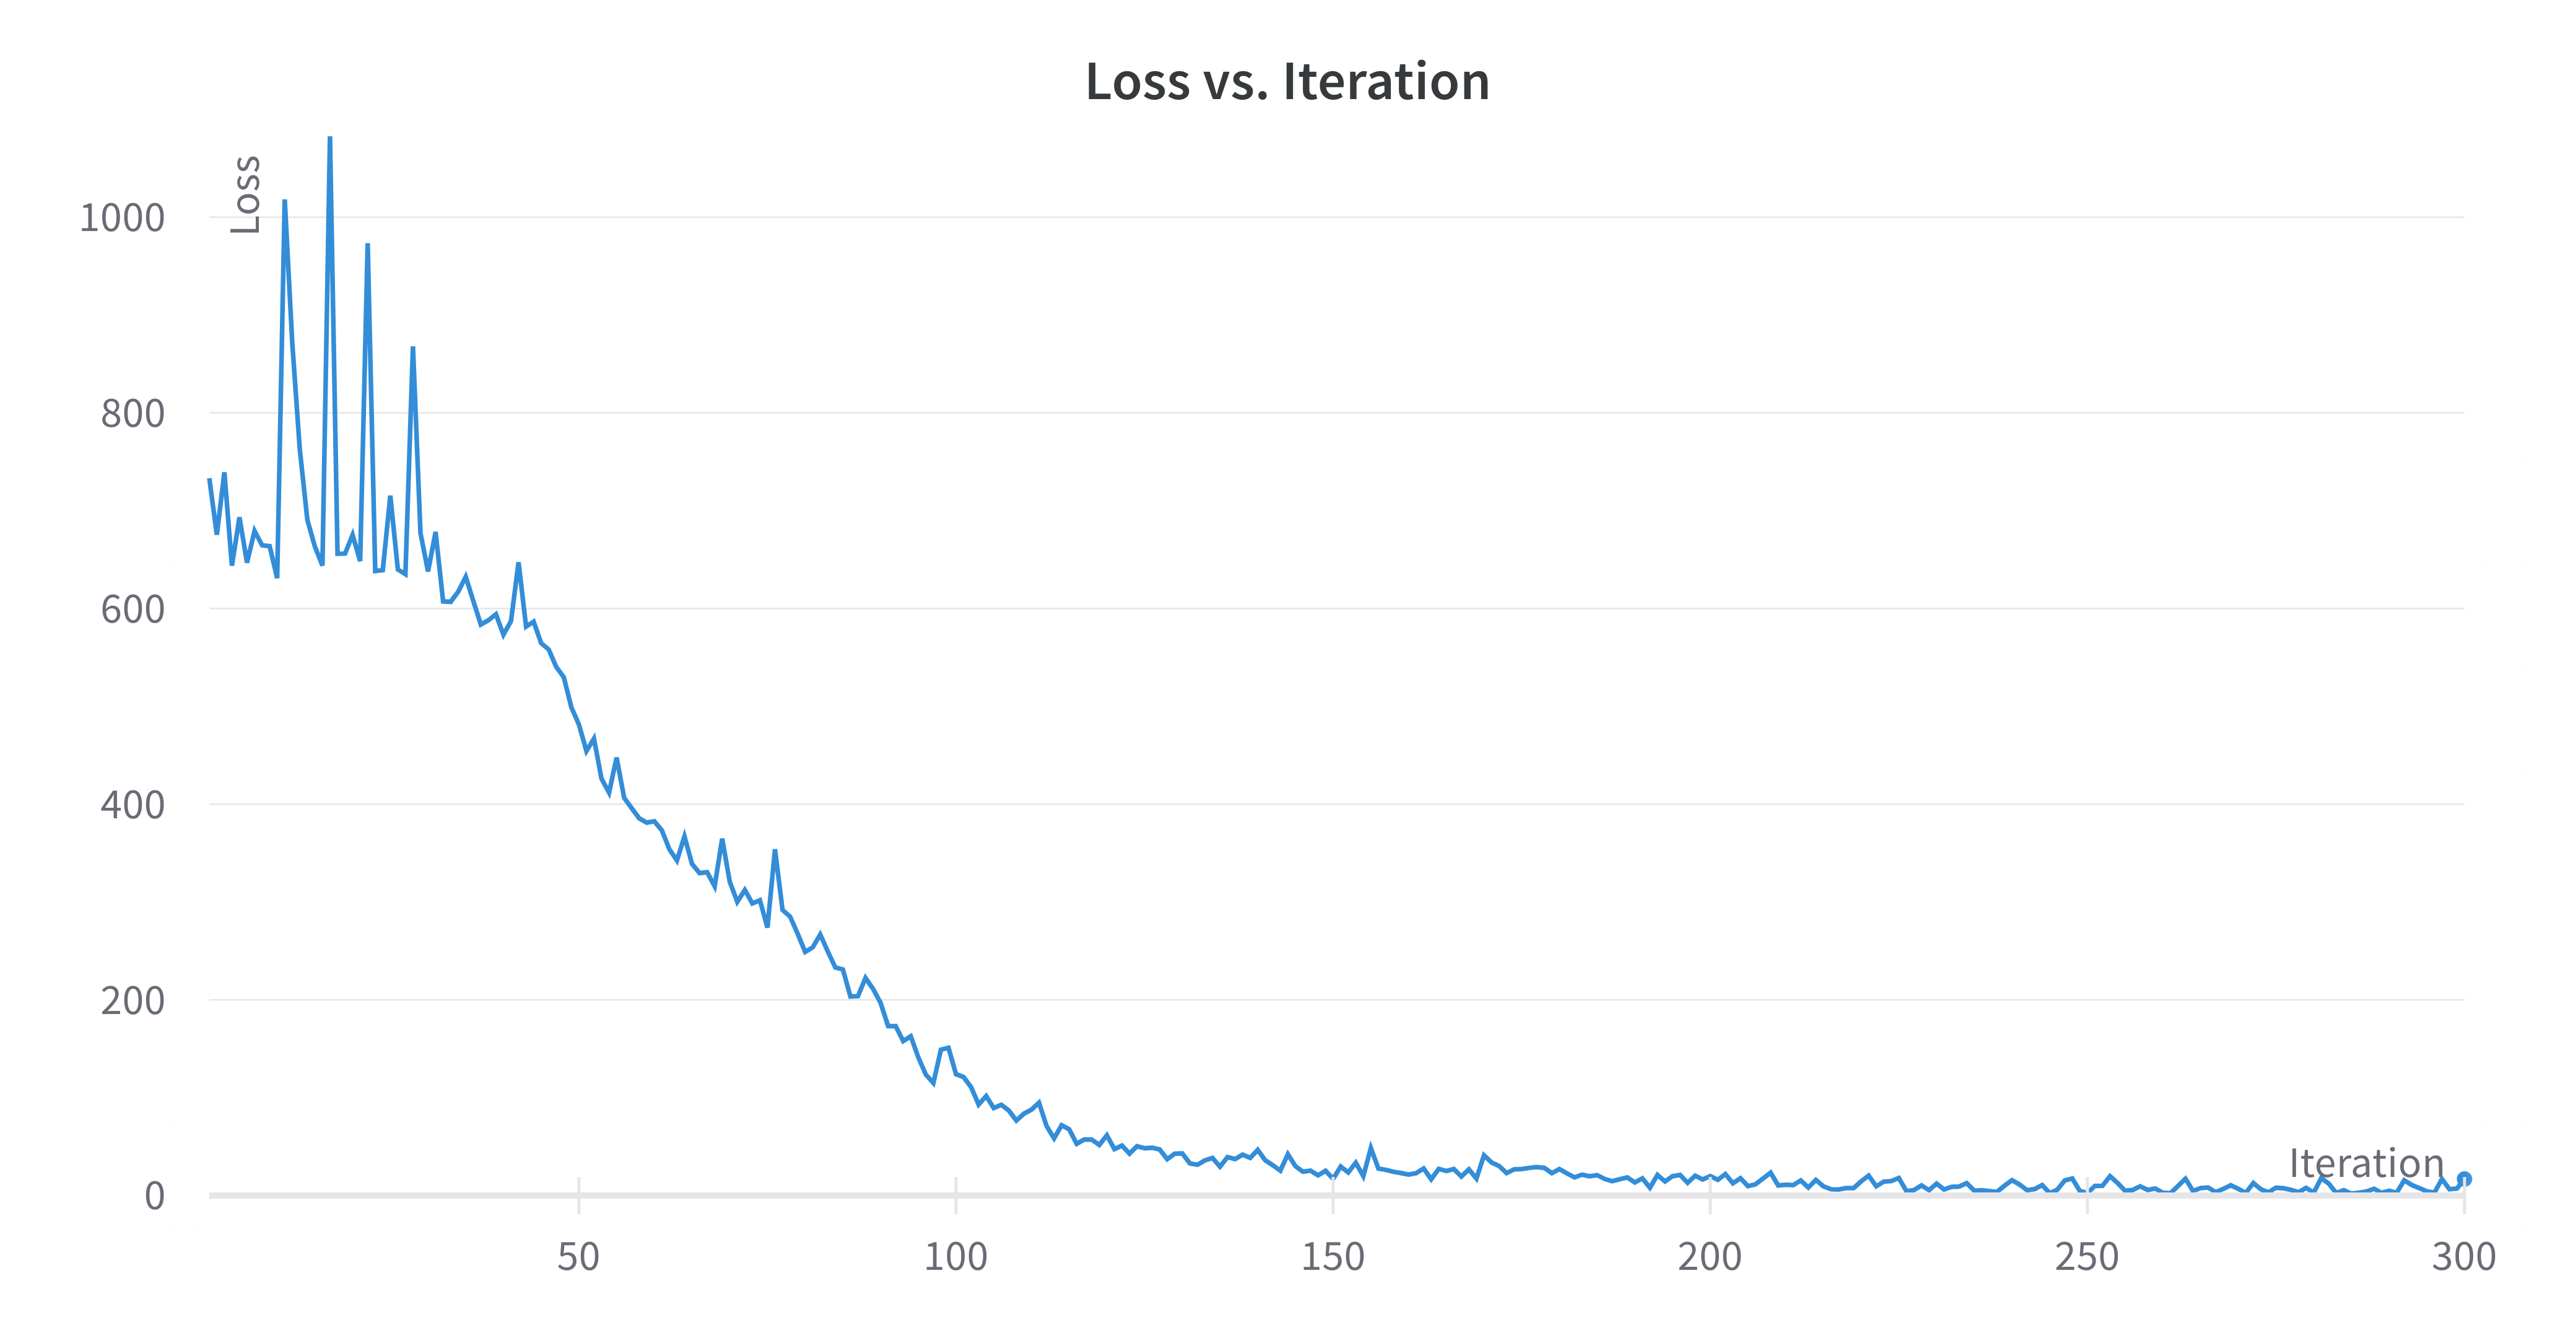
\includegraphics[width=0.6\textwidth]{images/attack_loss_iteration.png}
  \caption{CTC loss over 300 iterations of PGD.}
  \label{fig:attack_loss_iteration}
\end{figure}

\begin{figure}[h]
  \centering
  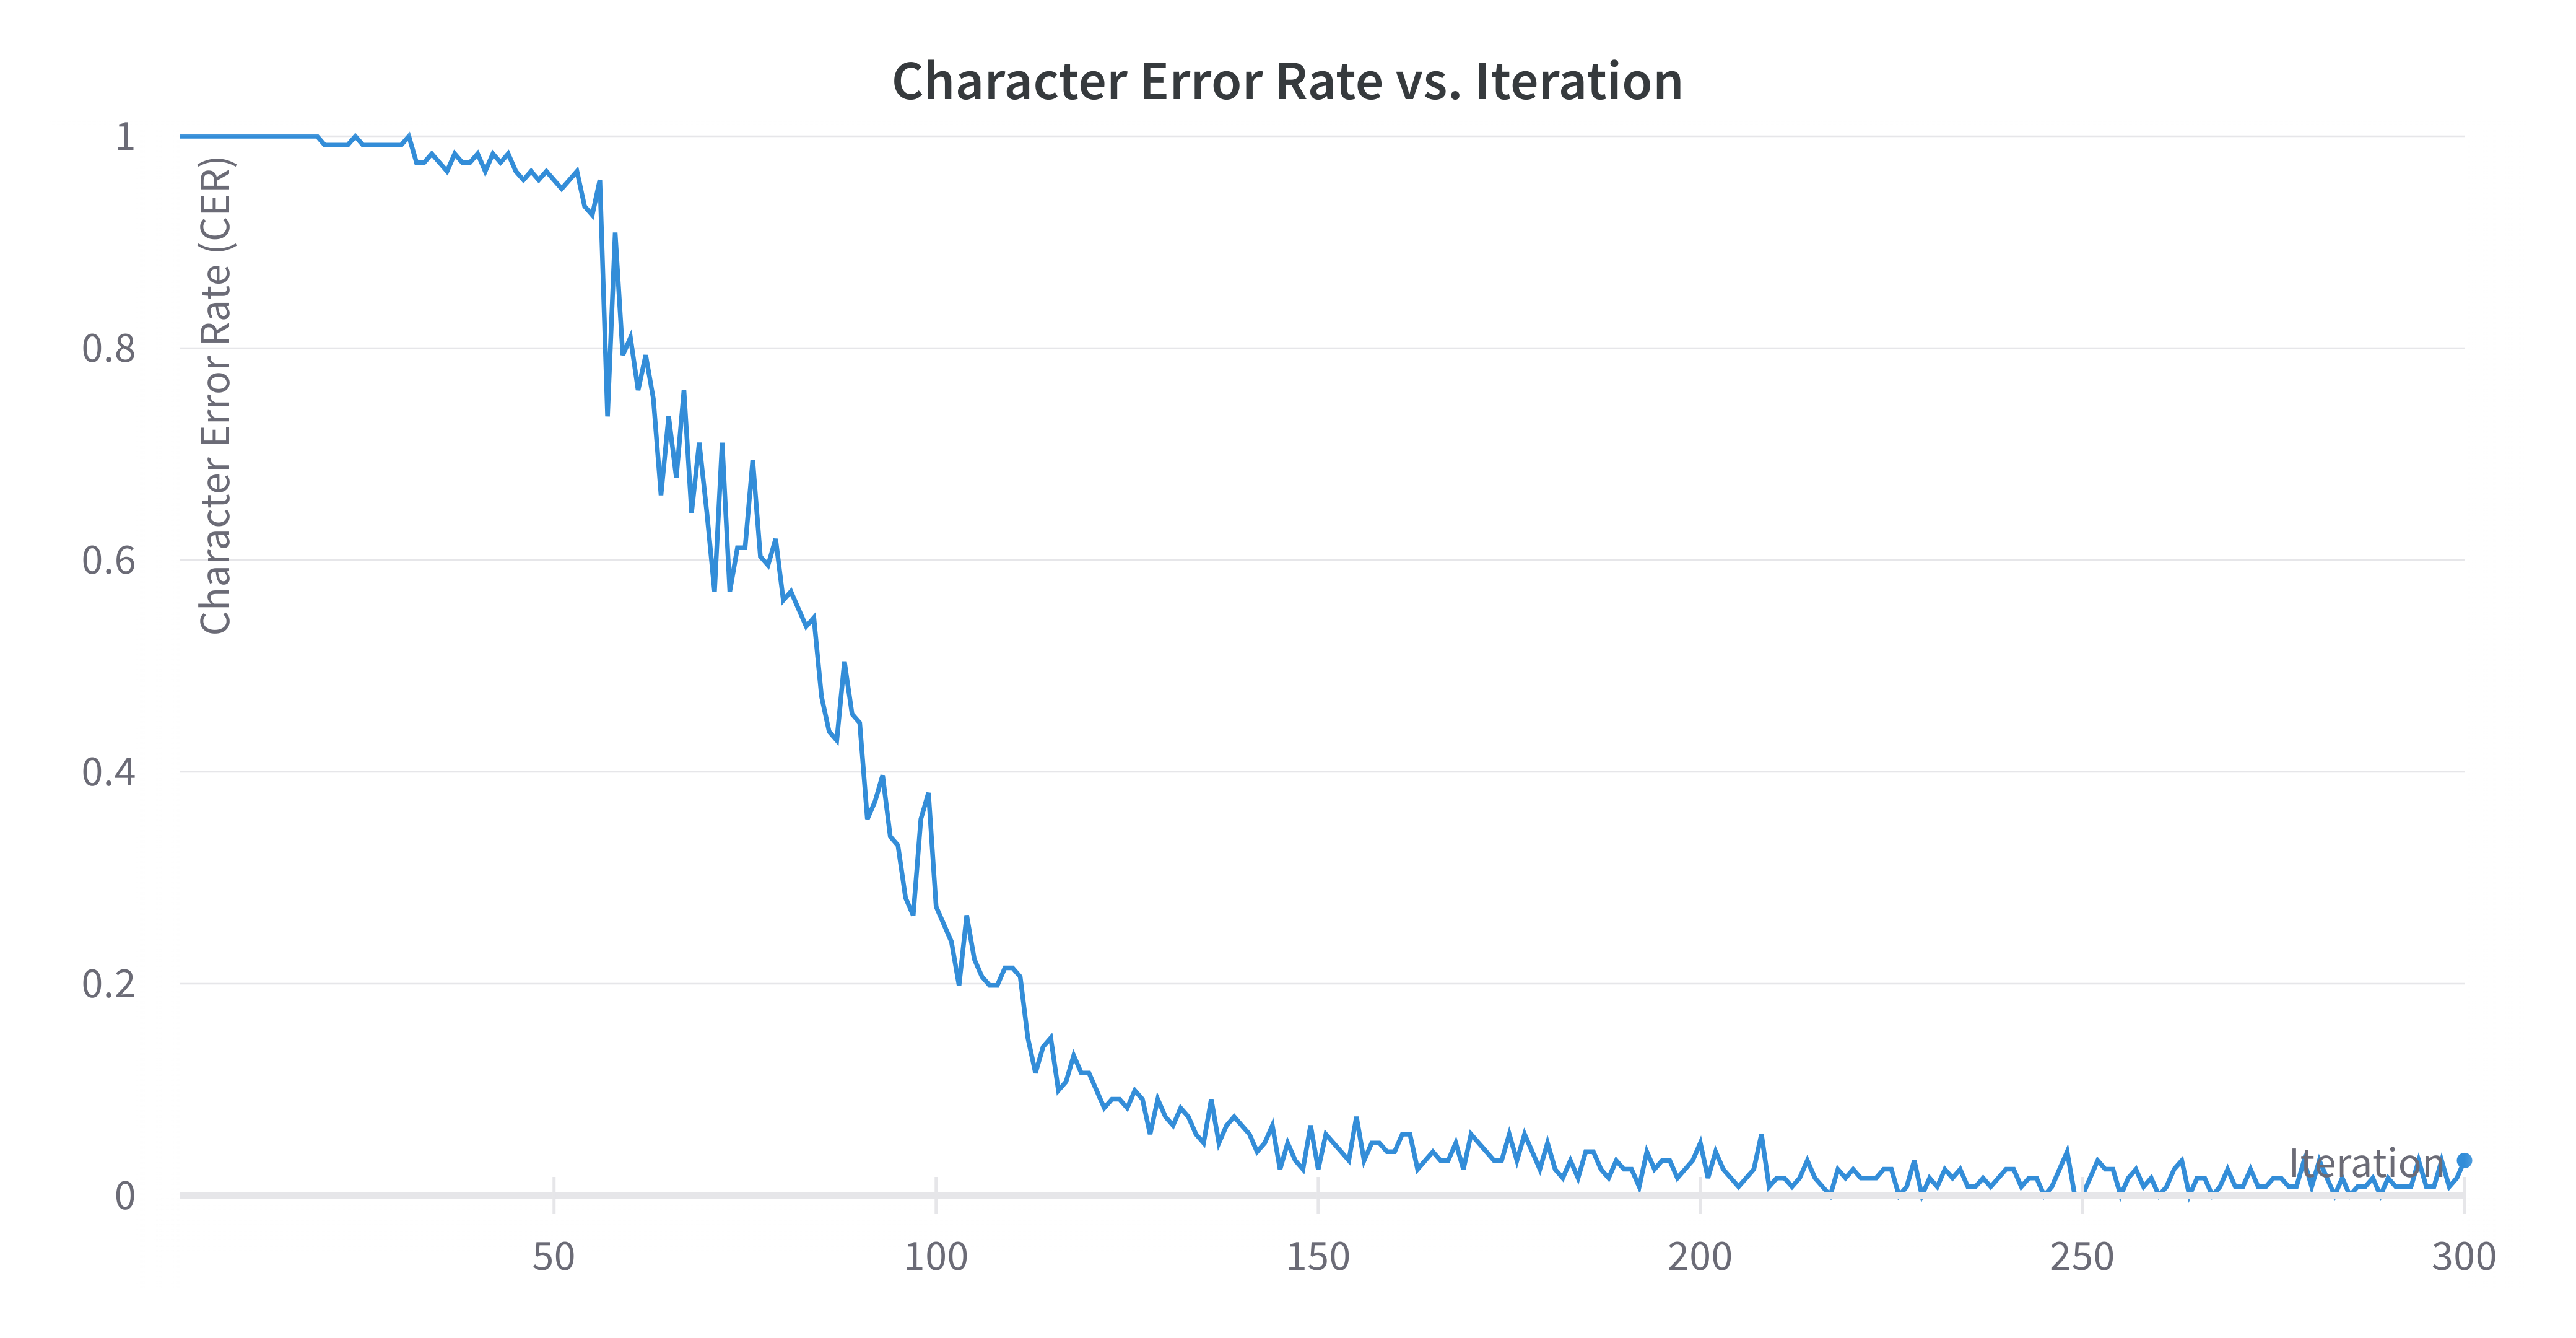
\includegraphics[width=0.6\textwidth]{images/attack_cer_iteration.png}
  \caption{Character Error Rate over 300 iterations of PGD.}
  \label{fig:attack_cer_iteration}
\end{figure}

When we look at the transcripts generated by the speech recognition model at
various iterations of PGD (\autoref{tab:attack_transcript}), we see that even by
iteration 150, the adversarial transcript is quite close to the target
transcript. By iteration 250, only one word has a typo and by iteration 300, the
adversarial transcript is only off by one letter.

\begin{table}[h]
  \centering
  \begin{tabularx}{\textwidth}{lX}
    \hline
    Iteration & Transcript \\
    \hline
    0         &            \\\\
    50        & \textbf{I} \textbf{CCON}     \\\\
    100       & \textbf{SEATTHE} \textbf{CENTE} \textbf{CKHAK} \textbf{TW} \textbf{THPEE} \textbf{LU} PIREP \textbf{TPEATUE} MINUS \textbf{UR} \textbf{COUD} \textbf{ASES} \textbf{THE} \textbf{THUAND} \textbf{HIGHT} \textbf{RN} \textbf{IC} \textbf{ACCATIN} \\\\
    150       & SEATTLE CENTER SKYHAWK TWO THREE ZULU PIREP \textbf{TEMPERAKTURE} \textbf{MAINUS} FOUR CLOUD BASES \textbf{THR} THOUSAND LIGHT RIME \textbf{KE} \textbf{ACCUMULATIN} \\\\
    200       & SEATTLE CENTER SKYHAWK TWO THREE ZULU PIREP \textbf{TEMPERARTURE} MINUS FOUR CLOUD BASES THREE \textbf{THTUSAND} LIGHT RIME ICE ACCUMULATION \\\\
    250       & SEATTLE CENTER SKYHAWK TWO THREE ZULU PIREP TEMPERATURE MINUS FOUR CLOUD BASES THREE THOUSAND LIGHT RIME \textbf{AKE} ACCUMULATION \\\\
    300       & SEATTLE CENTER SKYHAWK TWO THREE ZULU PIREP TEMPERATURE MINUS FOUR CLOUD BASES THREE THOUSAND LIGHT RIME ICE \textbf{ACCUMLATION} \\\\
    \hline
  \end{tabularx}
  \caption{Transcript of adversarial PIREP over 300 iterations of PGD. Words with typos are bolded.}
  \label{tab:attack_transcript}
\end{table}

Another interesting visualization of our method is the spectrogram of the intial
noise selected from \autoref{eq:noise} compared to the adversarial PIREP after
300 iterations of PGD (\autoref{fig:spectrograms}). In the bottom spectrogram,
we can visually see the result of our adversarial attack in the form of a
distinct pattern in the 0 to 3000 Hz frequency range. Although this pattern can
be seen on the spectrogram, it is not easily detectable by the human ear over
the static noise.

\begin{figure}[h]
  \centering
  \includegraphics[width=0.9\textwidth]{images/n}
  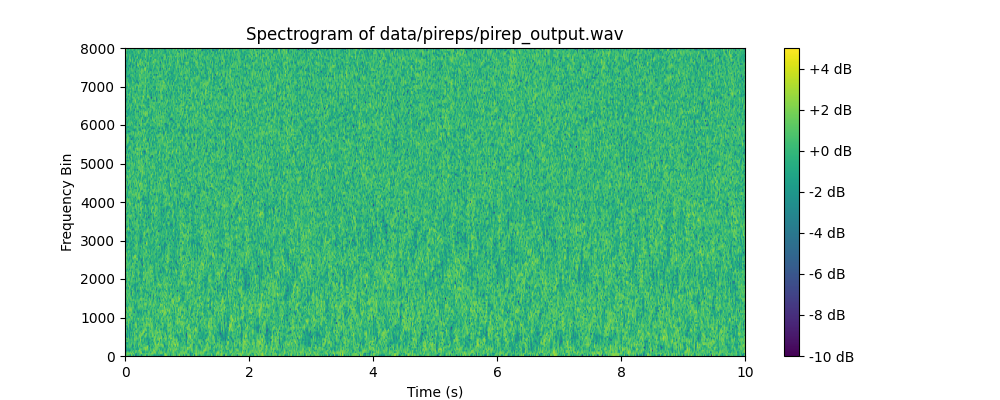
\includegraphics[width=0.9\textwidth]{images/pirep_output.png}
  \caption{\textit{Top}: Spectrogram showing randomly selected noise from \autoref{eq:noise}. \textit{Bottom}: Spectrogram showing adversarial PIREP after 300 iterations of PGD. Notice the formations in the 0 to 3000 Hz frequency range.}
  \label{fig:spectrograms}
\end{figure}

\section{Evaluation}

\subsection{Static Consequences}

Static interference poses significant challenges for flight traffic controllers when it comes to radio communication. 
This interference, often caused by atmospheric conditions or electromagnetic disturbances, can result in distorted
or garbled transmissions, making it difficult for controllers to receive and interpret crucial information from pilots. 
Static interference can lead to miscommunication, misunderstandings, and delays in coordinating flight operations. 
This posses a problem for our attack vector, if sufficient static is introduced into the system it can cause our attack to fail.

\subsection{Noise Injection}

\section{Defenses}

We suggest several methods for defending against our adversarial PIREPs. These
methods are proposed as a starting point for future research, and should be
evaluated in real-world settings before being deployed in safety-critical
systems.

\subsection{Noise Injection}

% TODO: evaluate noise injection on real PIREPs vs adversarial PIREPs
% If real PIREPs are more robust, then noise injection is a viable defense
% low Freq noise could in theory protect normal voice communication and get rid of static adversarial attacks

\subsection{Adversarial Detection Model}

% Detect adversarial PIREPs using a model trained on adversarial examples
% Using a different model architecture, such as a CNN, may be more challenging
% to attack (since the adversary would need to defeat both the CNN detection
% model and the speech recognition model).

\subsection{Gradual Implementation}

Finally, one of the simplest and most effective defenses against adversarial
attacks is a human in the loop. In the case of PIREPs, this may mean that an air
traffic controller would be responsible for reviewing the PIREP before it is
entered into the system. This would be a simple and effective defense against
our attack since a human would be able to easily classify the adversarial PIREP
as static. Although this does require additional effort from the air traffic
controller, it would likely still be less work than the current process of
transcribing the PIREP by hand, and thus still helpful in reducing the workload
of air traffic controllers.

\section{Conclusion}

\subsection{Future Work}

%--------------------------------
% Citations
%--------------------------------
\bibliography{report}

\end{document}

undefined